\chap{Timer Interrupt and LED Scanning}

\section{Introduction}
Timers are one of the most important features in modern micro-controllers. They allow us to measure how long something takes to execute, create non-blocking code, precisely control pin timing, and even run operating systems. In this manual, how to configure a timer using STM32CubeIDE is presented how to use them to flash an LED. Finally, students are proposed to finalize 10 exercises using timer interrupt for applications based LED Scanning.

\begin{figure}[!htp]
    \centering
    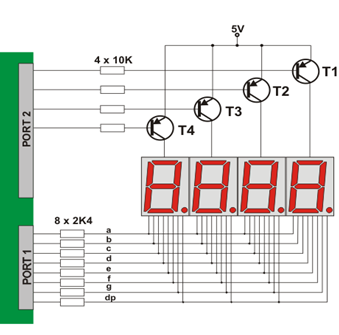
\includegraphics[width=3.5in]{source/picture/bai_2/led_scanning1.png}
    \caption{\textit{Four seven segment LED interface for a micro-controller}}
    \label{bai2_intro1}
\end{figure}


Design an interface for with multiple LED (seven segment or matrix) displays which is to be controlled is depends on the number of input and output pins needed for controlling all the LEDs in the given matrix display, the amount of current that each pin can source and sink and the speed at which the micro-controller can send out control signals. With all these specifications, interfacing can be done for 4 seven segment LEDs with a micro-controller is proposed in the figure above. \\


In the above diagram each seven segment display is having 8 internal LEDs, leading to the total number of LEDs is 32. However, not all the LEDs are required to turn ON, but one of them is needed. Therefore, only 12 lines are needed to control the whole 4 seven segment LEDs.   By controlling with the micro-controller, we can turn ON an LED during a same interval \textbf{$T_S$}. Therfore, the period for controlling all 4 seven segment LEDs is \textbf{$4T_S$}. In other words, these LEDs are scanned at frequecy \textbf{$f = 1 / 4T_S$}. Finally, it is obviously that if the frequency is greater than 30Hz (e.g. f = 50Hz), it seems that all LEDs are turn ON at the same time.\\

In this manual, the timer interrupt is used to design the interval $T_S$ for LED scanning. Unfortunately, the simulation on Proteus can not execute at high frequency, the frequency $f$ is set to a low value (e.g. 1Hz). In a real implementation, this frequency should be 50Hz.


\newpage
\section{Timer Interrupt Setup}
\textbf{Step 1: } Create a simple project, which LED connected to PA5. The manual can be found in the first lab.\\

\textbf{Step 2: } Check the clock source of the system on the tab \textbf{Clock Configuration} (from *.ioc file). In the default configuration, the internal clock source is used with 8MHz, as shown in the figure bellow.

\begin{figure}[!htp]
    \centering
    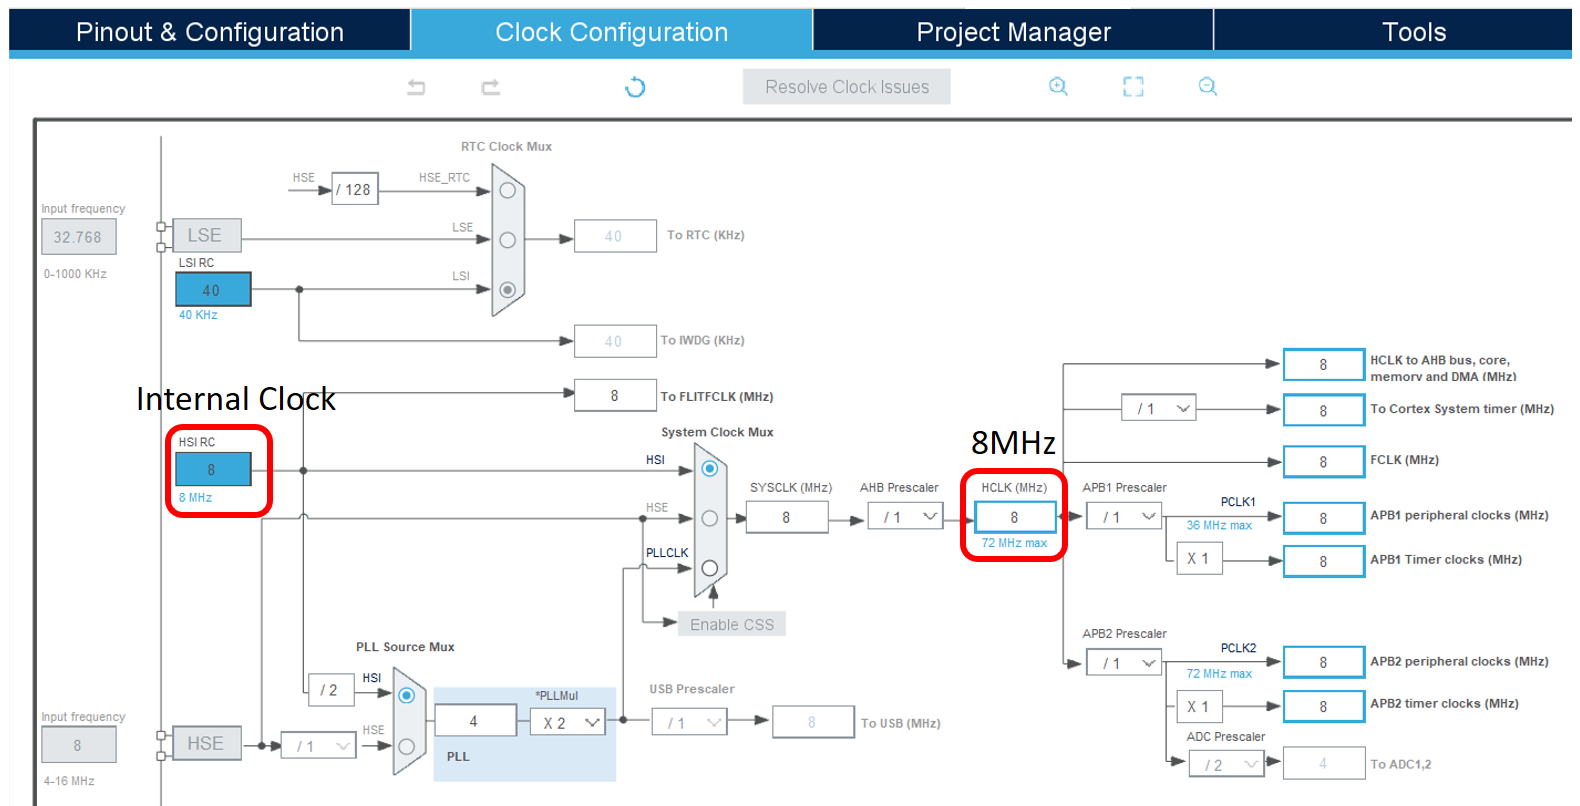
\includegraphics[width=5.5in]{source/picture/bai_2/lab2_m1.PNG}
    \caption{\textit{Default clock source for the system}}
    \label{bai2_m1}
\end{figure}

\textbf{Step 3: } Configure the timer on the \textbf{Parameter Settings}, as follows:
\begin{figure}[!htp]
    \centering
    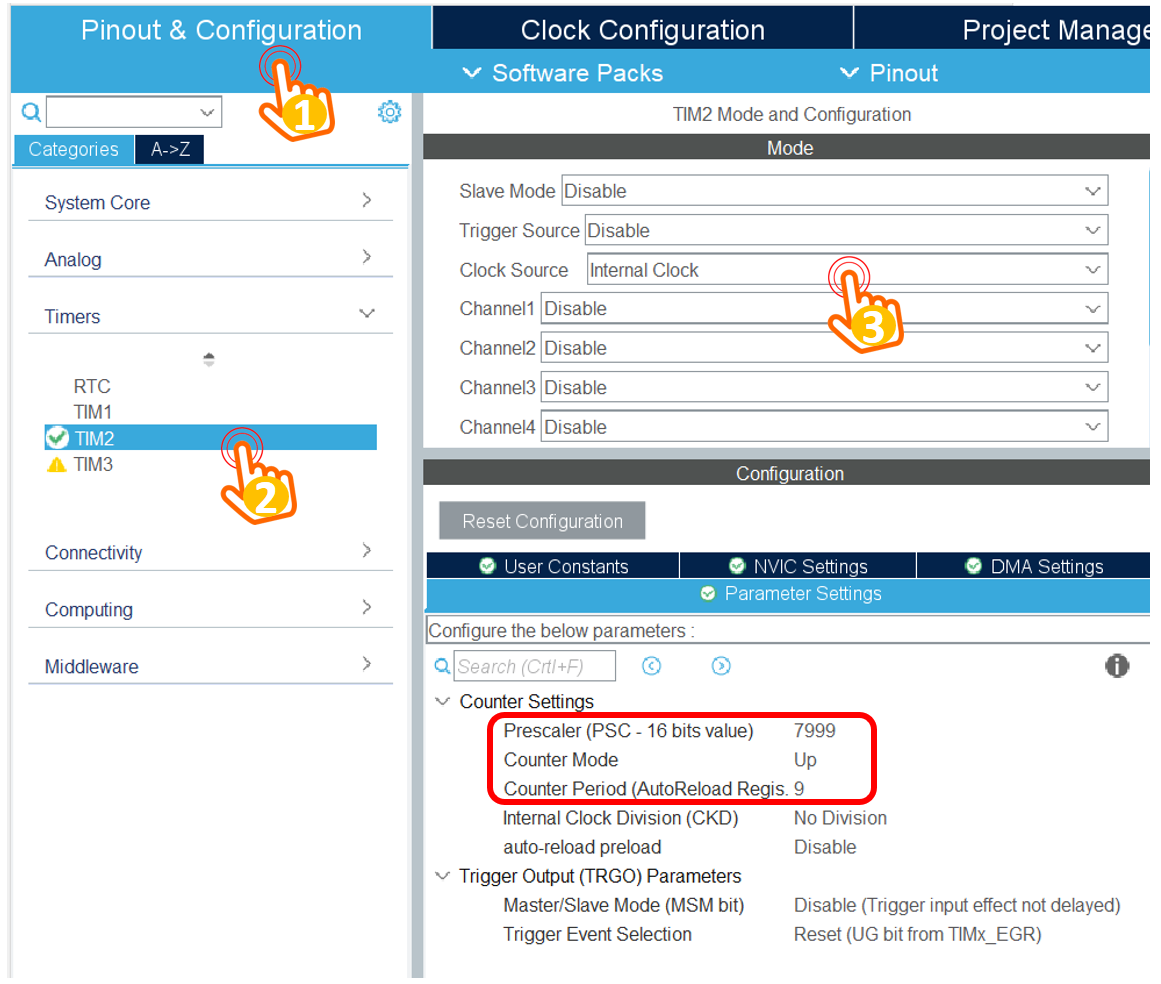
\includegraphics[width=3.5in]{source/picture/bai_2/lab2_m2.PNG}
    \caption{\textit{Configure for Timer 2}}
    \label{bai2_m2}
\end{figure}

Select the clock source for timer 2 to the \textbf{Internal Clock}. Finally, set the prescaller and the counter to 7999 and 9, respectively. These values are explained as follows:
\begin{itemize}
    \item The target is to set an interrupt timer to 10ms
    \item The clock source is 8MHz, by setting the prescaller to 7999, the input clock source to the timer is \textbf{8MHz/(7999+1) = 1000Hz}.
    \item The interrupt is raised when the timer counter is counted from 0 to 9, meaning that the frequency is divided by 10, which is 100Hz.
    \item The frequency of the timer interrupt is 100Hz, meaning that the period is \textbf{1/100Hz = 10ms}.
\end{itemize}

\textbf{Step 4: } Enable the timer interrupt by switching to \textbf{NIVC Settings} tab, as follows:

\begin{figure}[!htp]
    \centering
    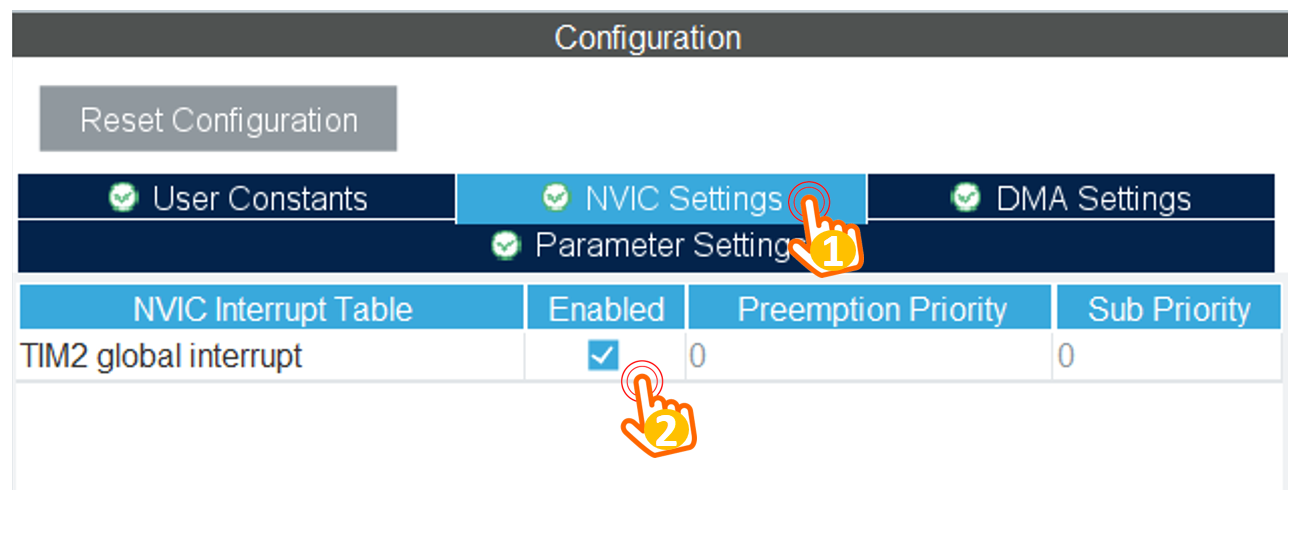
\includegraphics[width=4in]{source/picture/bai_2/lab2_m3.PNG}
    \caption{\textit{Enable timer interrupt}}
    \label{bai2_m3}
\end{figure}

Finally, save the configuration file to generate the source code.\\

\textbf{Step 5: } On the \textbf{main()} function, call the timer init function, as follows:

\begin{lstlisting}[caption=Init the timer interrupt in main]
int main(void)
{
  HAL_Init();
  SystemClock_Config();

  MX_GPIO_Init();
  MX_TIM2_Init();
  
  /* USER CODE BEGIN 2 */
  HAL_TIM_Base_Start_IT(&htim2);
  /* USER CODE END 2 */g3

  while (1){
  
  }
}
\end{lstlisting}

Please put the init function in a right place to avoid conflicts when code generation is executed (e.g. ioc file is updated).\\
\newpage
\textbf{Step 6: } Add the interrupt service routine function, this function is invoked every 10ms, as follows:

\begin{lstlisting}[caption=Add an interrupt service routine]
/* USER CODE BEGIN 4 */
void HAL_TIM_PeriodElapsedCallback(TIM_HandleTypeDef *htim){
	
}
/* USER CODE END 4 */
\end{lstlisting}

\textbf{Step 7: } To run a LED Blinky demo using interrupt, a short manual is presented as follows:
\begin{lstlisting}[caption=LED Blinky using timer interrupt]
/* USER CODE BEGIN 4 */
int counter = 100;
void HAL_TIM_PeriodElapsedCallback(TIM_HandleTypeDef *htim){
	counter--;
	if(counter <= 0){
		counter = 100;
		HAL_GPIO_TogglePin(LED_RED_GPIO_Port, LED_RED_Pin);
	}
}
/* USER CODE END 4 */
\end{lstlisting}

The \textbf{HAL\_TIM\_PeriodElapsedCallback} function is an infinite loop, which is invoked every cycle of the timer 2, in this case, is 10ms.\\



\newpage
\section{Exercise and Report}
\subsection{Exercise 1}
The first exercise show how to interface for multiple seven segment LEDs to STM32F103C6 micro-controller (MCU). Seven segment displays are common anode type, meaning that the anode of all LEDs are tied together as a single terminal and cathodes are left alone as individual pins. \\

In order to save the resource of the MCU, individual cathode pins from all the seven segment LEDs are connected together, and connect to 7 pins of the MCU. These pins are popular known as the \textbf{signal pins}. Meanwhile, the anode pin of each seven segment LEDs are controlled under a power enabling circuit, for instance, an PNP transistor. At a given time, only one seven segment LED is turned on. However, if the delay is small enough, it seems that all LEDs are enabling. \\

Implement the circuit simulation in Proteus with two 7-SEGMENT LEDs as following:

\begin{figure}[!htp]
    \centering
    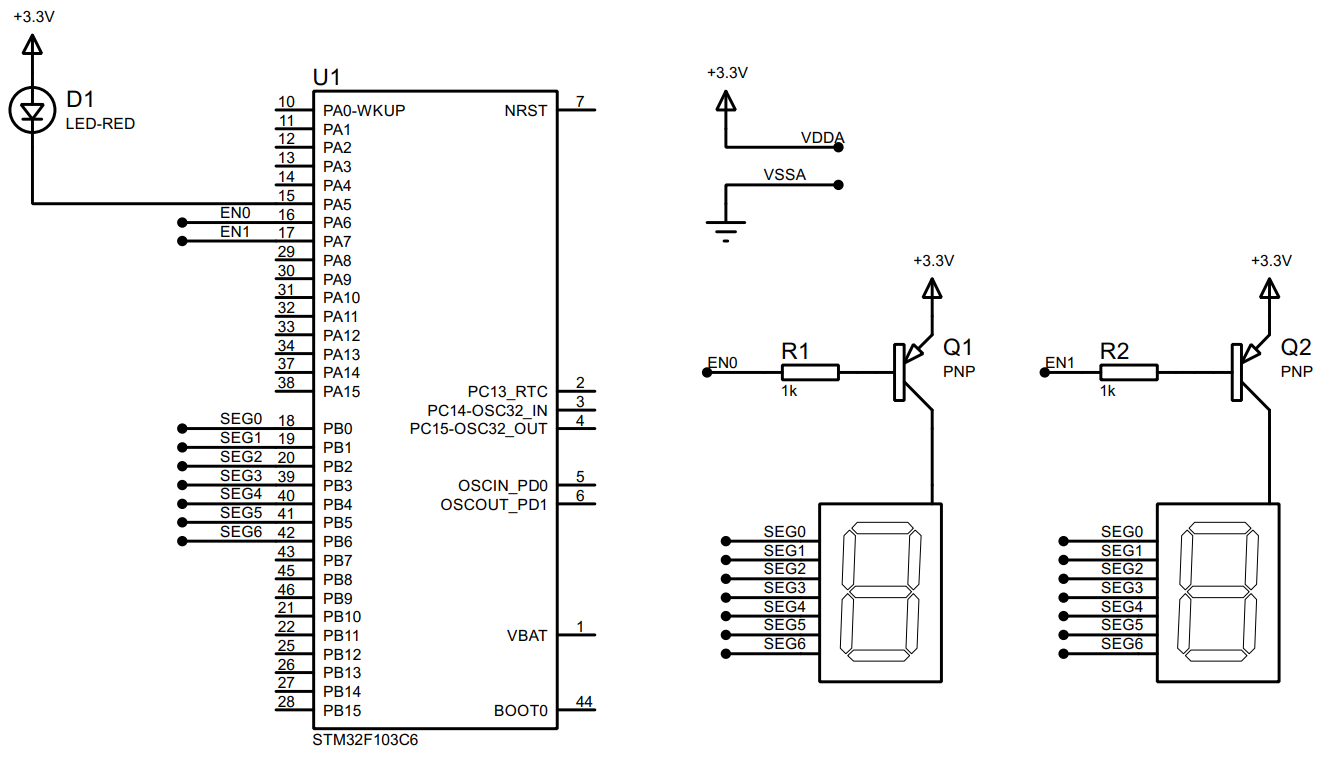
\includegraphics[width=5.5in]{source/picture/bai_2/lab2_ex1a.PNG}
    \caption{\textit{Simulation schematic in Proteus}}
    \label{bai2_pic1a}
\end{figure}
Components used in the schematic are listed bellow:
\begin{itemize}
    \item 7SEG-COM-ANODE (connected from PB0 to PB6)
    \item LED-RED
    \item PNP
    \item RES
    \item STM32F103C6
\end{itemize}


Students are proposed to use the function \textbf{display7SEG(int num)} in the Lab 1 in this exercise. Implement the source code in the interrupt callback function to display number \textbf{"1"} on the first seven segment and number \textbf{"2"} for second one. The switching time between 2 LEDs is half of second. \\

\textbf{Report 1: } Capture your schematic from Proteus and show in the report.\\

\textbf{Report 2: } Present your source code in the \textbf{HAL\_TIM\_PeriodElapsedCallback} function.\\

\textbf{Short question: } What is the frequency of the scanning process?\\

\subsection{Exercise 2}
Extend to 4 seven segment LEDs and two LEDs (connected to PA4, labeled as \textbf{DOT}) in the middle as following:

\begin{figure}[!htp]
    \centering
    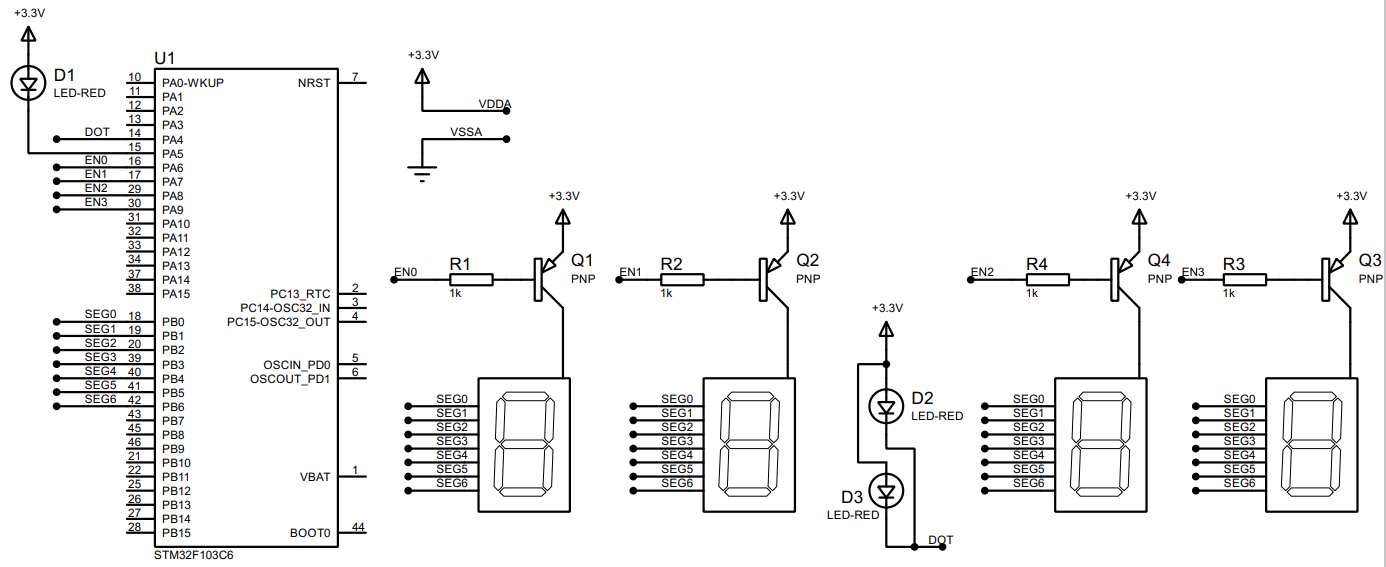
\includegraphics[width=5.5in]{source/picture/bai_2/lab2_ex2a.PNG}
    \caption{\textit{Simulation schematic in Proteus}}
    \label{bai2_pic1a}
\end{figure}

Blink the two LEDs every second. Meanwhile, number 3 is displayed on the third seven segment and number 0 is displayed on the last one (to present 12 hour and a half). The switching time for each seven segment LED is also a half of second (500ms). \textbf{Implement your code in the timer interrupt function.}\\

\textbf{Report 1: } Capture your schematic from Proteus and show in the report.\\

\textbf{Report 2: } Present your source code in the \textbf{HAL\_TIM\_PeriodElapsedCallback} function.\\

\textbf{Short question: } What is the frequency of the scanning process?\\

\subsection{Exercise 3}
Implement a function named \textbf{update7SEG(int index)}. An array of 4 integer numbers are declared in this case. The code skeleton in this exercise is presented as following:
\newpage
\begin{lstlisting}[caption=An example for your source code]
const int MAX_LED = 4;
int index_led = 0;
int led_buffer[4] = {1, 2, 3, 4};
void update7SEG(int index){
    switch (index){
        case 0:
            //Display the first 7SEG with led_buffer[0]
            break;
        case 1:
            //Display the second 7SEG with led_buffer[1]
            break;
        case 2:
            //Display the third 7SEG with led_buffer[2]
            break;
        case 3:
            //Display the forth 7SEG with led_buffer[3]
            break;
        default:
            break;
    }
}
\end{lstlisting}

This function should be invoked in the timer interrupt, e.g update7SEG(index\_led++). The variable \textbf{index\_led} is updated to stay in a valid range, which is from 0 to 3. \\

\textbf{Report 1: } Present the source code of the update7SEG function. \\

\textbf{Report 2: } Present the source code in the HAL\_TIM\_PeriodElapsedCallback.\\

Students are proposed to change the values in the \textbf{led\_buffer} array for unit test this function, which is used afterward.

\subsection{Exercise 4}
Change the period of invoking update7SEG function in order to set the frequency of 4 seven segment LEDs to 1Hz. The DOT is still blinking every second.\\


\textbf{Report 1: } Present the source code in the \textbf{HAL\_TIM\_PeriodElapsedCallback}. \\

\subsection{Exercise 5}
Implement a digital clock with \textbf{hour} and \textbf {minute} information displayed by 2 seven segment LEDs. The code skeleton in the \textbf{main} function is presented as follows:
\begin{lstlisting}[caption=An example for your source code]
int hour = 15, minute = 8, second = 50;

while(1){
    second++;
    if (second >= 60){
        second = 0;
        minute++;
    }
    if(minute >= 60){
        minute = 0;
        hour++;
    }
    if(hour >=24){
        hour = 0;
    }
    updateClockBuffer();
    HAL_Delay(1000);
}
\end{lstlisting}

The function \textbf{updateClockBuffer} will generate values for the array \textbf{led\_buffer} according to the values of hour and minute. In the case these values are 1 digit number, digit 0 is added. \\

\textbf{Report 1: } Present the source code in the \textbf{updateClockBuffer} function.

\subsection{Exercise 6}
The main target from this exercise to reduce the complexity (or reduce code processing) in the timer interrupt. The time consumed in the interrupt can lead to the nested interrupt issue, which can crash the whole system. A simple solution can disable the timer whenever the interrupt occurs, the enable it again. However, the real-time processing is not guaranteed anymore.\\

In this exercise, a software timer is created and its counter is count down every timer interrupt is raised (every 10ms). By using this timer, the \textbf{Hal\_Delay(1000)} in the main function is removed. In a MCU system, non-blocking delay is better than blocking delay. The details to create a software timer are presented bellow. The source code is added to your current program, \textbf{do not delete the source code you have on Exercise 5.}\\

\textbf{Step 1: } Declare variables and functions for a software timer, as following:
\begin{lstlisting}[caption=Software timer based timer interrupt]
/* USER CODE BEGIN 0 */
int timer0_counter = 0;
int timer0_flag = 0;
int TIMER_CYCLE = 10;
void setTimer0(int duration){
	timer0_counter = duration /TIMER_CYCLE;
	timer0_flag = 0;
}
void timer_run(){
	if(timer0_counter > 0){
		timer0_counter--;
		if(timer0_counter == 0) timer0_flag = 1;
	}
}
/* USER CODE END 0 */
\end{lstlisting}

Please change the \textbf{TIMER\_CYCLE} to your timer interrupt period. In the manual code above, it is \textbf{10ms}. \\

\textbf{Step 2: } The \textbf{timer\_run()} is invoked in the timer interrupt as following:

\begin{lstlisting}[caption=Software timer based timer interrupt]
void HAL_TIM_PeriodElapsedCallback(TIM_HandleTypeDef *htim){
	
	timer_run();
	
	//YOUR OTHER CODE
}
\end{lstlisting}

\textbf{Step 3: } Use the timer in the main function by invoked setTimer0 function, then check for its flag (timer0\_flag). An example to blink an LED connected to PA5 using software timer is shown as follows:
\begin{lstlisting}[caption=Software timer is used in main fuction to blink the LED]
setTimer0(1000);
while (1){
    if(timer0_flag == 1){
        HAL_GPIO_TogglePin(LED_RED_GPIO_Port, LED_RED_Pin);
        setTimer0(2000);
    }
}
\end{lstlisting}

\textbf{Report 1: } if in line 1 of the code above is miss, what happens after that and why?\\


\textbf{Report 2: } if in line 1 of the code above is changed to setTimer0(1), what happens after that and why?\\

\textbf{Report 3: } if in line 1 of the code above is changed to setTimer0(10), what is changed compared to 2 first questions and why?\\

\subsection{Exercise 7}
Upgrade the source code in Exercise 5 (update values for hour, minute and second) by using the software timer and remove the HAL\_Delay function at the end. Moreover, the DOT (connected to PA4) of the digital clock is also moved to main function. \\

\textbf{Report 1: } Present your source code in the while loop on main function.

\subsection{Exercise 8}
Move also the update7SEG() function from the interrupt  timer to the main. Finally, the timer interrupt only used to handle  software timers. All processing (or complex computations) is move to an infinite loop on the main function, optimizing the complexity of the interrupt  handler function.\\

\textbf{Report 1: } Present your source code in the the main function. In the case more extra functions are used (e.g. the second software timer), present them in the report as well.

\subsection{Exercise 9}

This is an extra works for this lab. A LED Matrix is added to the system. A reference design is shown in figure bellow:
\begin{figure}[!htp]
    \centering
    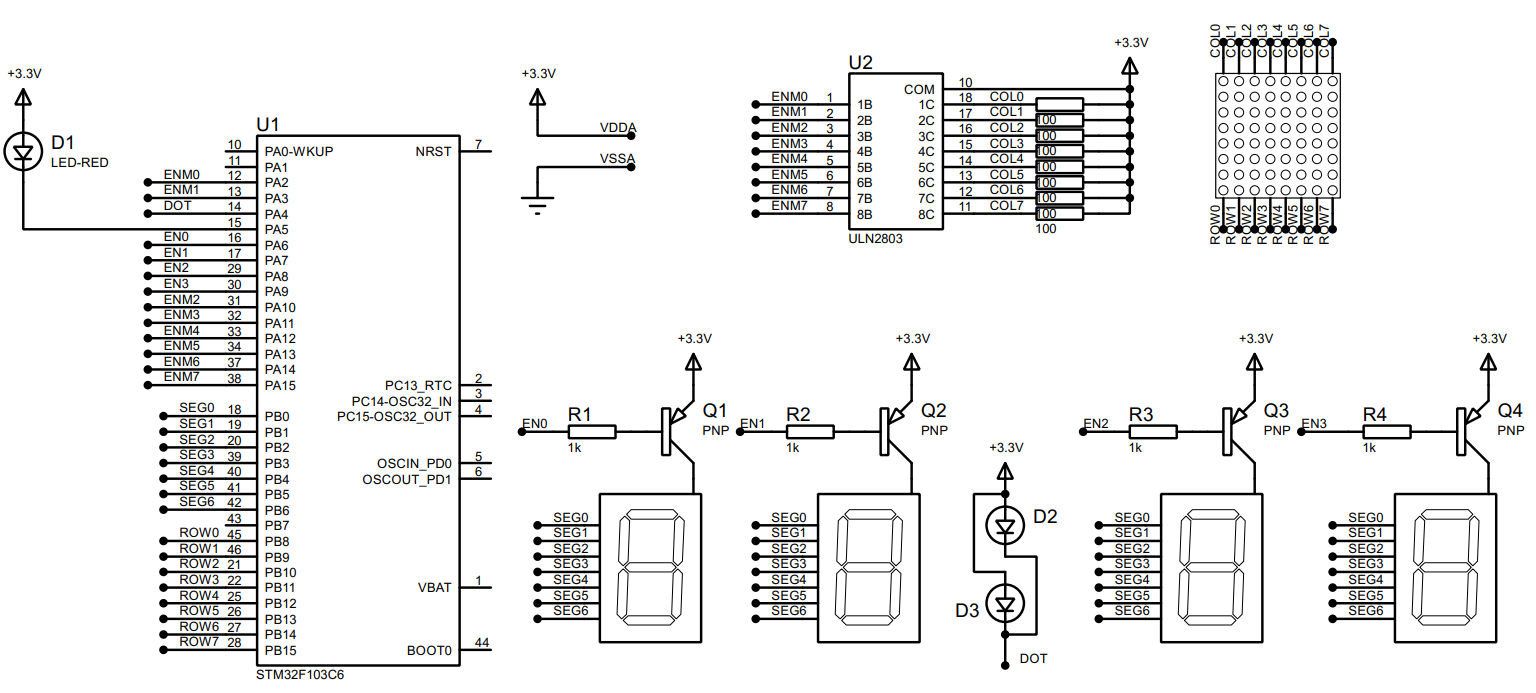
\includegraphics[width=5.5in]{source/picture/bai_2/lab2_m4.PNG}
    \caption{\textit{LED matrix is added to the simulation}}
    \label{bai2_pic9}
\end{figure}

In this schematic, two new components are added, including the \textbf{MATRIX-8X8-RED} and \textbf{ULN2803}, which is an NPN transistor array to enable the power supply for a column of the LED matrix. Students can change the enable signal (from ENM0 to  ENM7) if needed. Finally, the data signal (from ROW0 to ROW7) is connected to PB8 to PB15. \\

\textbf{Report 1: } Present the schematic of your system by capturing the screen in Proteus.\\

\textbf{Report 2: } Implement the function, updateLEDMatrix(int index), which is similarly  to 4 seven led segments.

\begin{lstlisting}[caption=Function to display data on LED Matrix]
const int MAX_LED_MATRIX = 8;
int index_led_matrix = 0;
uint8_t matrix_buffer[8] = {0x01, 0x02, 0x03, 0x04, 0x05, 0x06, 0x07, 0x08};
void updateLEDMatrix(int index){
    switch (index){
        case 0:
            break;
        case 1:
            break;
        case 2:
            break;
        case 3:
            break;
        case 4:
            break;
        case 5:
            break;
        case 6:
            break;
        case 7:
            break;
        default:
            break;
    }
}
\end{lstlisting}

Student are free to choose the invoking frequency of this function. However, this function is supposed to invoked in main function. Finally, please update the \textbf{matrix\_buffer} to display character \textbf{"A"}.

\subsection{Exercise 10}
Create an animation on LED matrix, for example, the character is shifted to the left. 

\textbf{Report 1: } Briefly describe your solution and present your source code in the report.
